
As outlined in Section~\ref{sec:introduction}, we refer by trending to the consistency of an observed change with the change issued by another measurement, a nowcast or a forecast.
In this section, we want to specify trending and lay out different methods of measuring and visualizing trending. 
In general, trending can be assessed for different lags $l$ separately, and the relevance of considered lags has to be determined based on the question at hand.
In Section~\ref{sec:notation}, the time series of differences $\diffx$ and $\diffy$ were introduced.
Whereas the computation of $\diffx$ differs in the different contexts, the trending assessment is similar.
In the following, we omit the difference's lag $l$ for the ease of notation; $\diffx$ and $\diffy$ refer to $\diffxl$ and $\diffyl$ for a common lag $l$.
Similarly, we call a measurement, nowcast, or forecast a \textit{prediction} for the quantity of interest $y$. \unsure{Discuss}
The remainder of the section is structured as follows.
Section~\ref{subsec:trending-basics} introduces trending basics and visualizes trending in a synthetical example.
Section~\ref{subsec:trending-measures} reviews conveyed quantification approaches from other fields.
The approaches are extended to the trending setting in Section~\ref{subsec:trending-noise}.
Section~\ref{subsec:trending-cond-prob} introduces a new graphical method of trending assessment.
Section~\ref{subsec:trending-bootstrap} gives bootstrap methods for computing confidence intervals for the measures and conductes a simulation study on their properties.


\subsection{Basics of trending and four-quadrant plots}\label{subsec:trending-basics}

As noted above, a prediction is trending perfectly if all occurred changes are predicted correctly, that is, the sign of all elements of $\diffx$ and $\diffy$ coincide.
Perfect trending is hardly the case in practice, but a weaker requirement is needed.
Accordingly, when assessing the trending, we examine the statistical consistency of $\sign(\diffx)$ and $\sign(\diffy)$.
A simple yet insightful method is the four-quadrant plot.
For example, it is known in cardiac output measurement analysis~\parencite{Saugel2015}. \todo{Add other citations}
Thereby, the occurred changes are plotted together with the predicted changes, that is, $(\diffy_t, \diffx_t)$ for $t = 1, \dots, T$.
Thus, the x-axis of a four-quadrant plot shows the true value differences, whereas the y-axis displays prediction data differences.
Points in the green upper right and lower left quadrant reflect a correct trending for the respective time step, whereas point in the remaining red quadrants show incorrect predicted changes.
Figure~\ref{fig:trending_basic_4q} displays a basic four-quadrant plot.
Points 2, 3, 5, and 6 show trending, whereas points 1, 4, and 7 count for anti-trending behavior.
Figure~\ref{fig:trending_basic_4q_sample} shows a four-quadrant plot for a more extensive simulated data set with $T=1461$, for example, four years of daily data.
The data generation is described in Appendix~\ref{sec:app-trending-data-generation} and will carry through this section.
The four-quadrant plot resembles a butterfly-like shape, with more data in the upper right and lower left quadrants than in the remaining quadrants.
The four-quadrant plot is intuitive to interpret, and the magnitude and direction of change are shown simultaneously.
It can be extended by including information on the date of difference in the point color.
In Figure~\ref{fig:trending_basic_4q_sample_color}, blue points refer to small time indices and turn green for larger $t$.
However, four-quadrant plots become crowded for larger datasets, and the sequential information on the differences is complex to assess thoroughly.
There are other visualization techniques, such as polar plots or the Bland-Altmann analysis.
However, they lack the clearness and intuition of the four-quadrant plot while adding no more information on the trending~\parencite{Saugel2015}.

\begin{figure}
\centering
\begin{subfigure}[t]{.24\textwidth}
\includegraphics{plots/illustrative_examples/4Q_without_excl}
\caption{Basic four-quadrant plot.} \label{fig:trending_basic_4q}
\end{subfigure}\hspace{0.01\textwidth}%
\begin{subfigure}[t]{.24\textwidth}
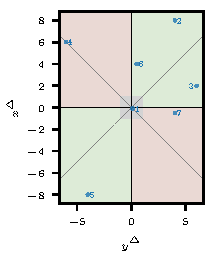
\includegraphics{plots/illustrative_examples/4q_excl_box}
\caption{Four-quadrant plot with rectangle exclusion area.}\label{fig:trending_basic_4q_excl_box}
\end{subfigure}\hspace{0.01\textwidth}%
\begin{subfigure}[t]{.24\textwidth}
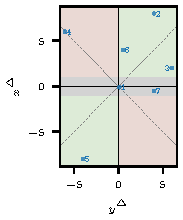
\includegraphics{plots/illustrative_examples/4q_excl_axis}
\caption{Four-quadrant plot with horizontal exclusion area.} \label{fig:trending_basic_4q_excl_axis}
\end{subfigure}\hspace{0.01\textwidth}%
\begin{subfigure}[t]{.24\textwidth}
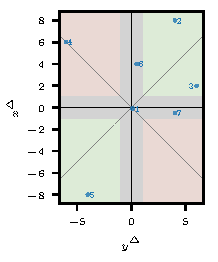
\includegraphics{plots/illustrative_examples/4q_excl_cross}
\caption{Four-quadrant plot with crossed exclusion area.}\label{fig:trending_basic_4q_excl_cross}
\end{subfigure}%
\caption{Illustrations of the four-quadrant plot with sample points and with and without exclusion areas. }
\label{fig:trending_4q}
\end{figure}

\subsection{Trending ratio and other measures}\label{subsec:trending-measures}

Analyzing the number of points in the green quadrants versus the red quadrants boils down to assessing the probability of trending $P(\diffxrv \diffyrv > 0)$.
Note that $z_1 z_2 > 0$ if and only if $\sign(z_1) = \sign(z_2)$ ($z_1, z_2 \in \R$).
To estimate $P(\diffxrv \diffyrv > 0)$ it lies at hand to use
\begin{equation}
    \acc (\diffx, \diffy) \coloneqq \frac{\sum_{t \in \mathcal{T}} \ind{\diffx \diffy > 0}}{\card{T}}.\label{eq:acc}
\end{equation}
We refer to this estimator as the trending ratio of the prediction and set $\mathcal{T} = \{1, \dots, T\}$.
Visually, the measure computes the fraction of points in the upper right or lower left quadrant.
Such a $2 \times 2$ table of counts is often called a contingency table and is often used in other scientific areas for evaluation, for example, in dichotomous forecasting or as a confusion matrix in classification analysis~\parencites(see, e.g., the introductions in)()[Ch. 4]{James2021}[Ch. 3]{Jolliffe2012}.
There, a wide range of other methods is usually used to analyze further characteristics of contingency tables.
Two simple measures focusing on specific areas of interest are the positive and negative trending ratio $\accp$ and $\accm$, respectively.
They are defined as
\begin{align}
    \accp (\diffx, \diffy) &\coloneqq \frac{\sum_{t \in \mathcal{T}} \ind{\diffxt \diffyt > 0} \ind{\diffxt > 0}}{\sum_{t \in \mathcal{T}} \ind{\diffxt > 0}} \label{eq:accp}\\
    \accm (\diffx, \diffy) &\coloneqq \frac{\sum_{t \in \mathcal{T}} \ind{\diffxt \diffyt > 0} \ind{\diffxt < 0}}{\sum_{t \in \mathcal{T}} \ind{\diffxt < 0}}\label{eq:accm}
\end{align}
In the classification context, these measures are known as positive or negative predictive value and hit rate or detection failure ratio in forecasting.
The two give estimates of $P(\diffxrv \diffyrv > 0 | \diffxrv > 0)$ and $P(\diffxrv \diffyrv > 0 | \diffxrv < 0)$, respectively.
There are various adapted measures for unbalanced outcomes, for example, Cohen's $\kappa$ \todo{Citation}.
Cohen's $\kappa$ reduces to rescaling the trending ratio in the case of a $2\times2$ table and balanced outcomes.
Unbalanced outcomes of the differences are unlikely in our setting as they are obtained from differencing time series data.
Nevertheless, if in a four-quadrant plot the number of positive and negative $\diffy$ are observed to differ widely, one should consider another as measures such as Cohen's $\kappa$ or the ones listed in \textcite[Table 3.3]{Jolliffe2012}.

All measures can also be evaluated as a rolling estimate to detect changes in performance over time.
Figure~\ref{fig:trending_ratio_time_series} depicts a rolling window estimate of the trending ratio for the simulated data of Figures~\ref{fig:trending_basic_4q_sample} and \ref{fig:trending_basic_4q_sample_color}.
Thus, the yearly course of the prediction's trending ratio can be detected.
This trade cannot be observed in the two four-quadrant plot as it is overlaid by the high number of points.

\begin{figure}
    \centering
    \begin{subfigure}[t]{.24\textwidth}
\includegraphics{plots/illustrative_examples/4Q_sample_without_time}
\caption{Four-quadrant plot with simulated data.}\label{fig:trending_basic_4q_sample}
\end{subfigure}%
\begin{subfigure}[t]{.24\textwidth}
\includegraphics{plots/illustrative_examples/4Q_sample_with_time}
\caption{The data is colored according to the time index $t$, the greener, the later.}\label{fig:trending_basic_4q_sample_color}
\end{subfigure}%
\begin{subfigure}[t]{.48\textwidth}
    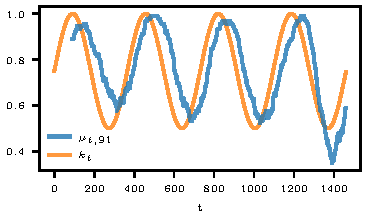
\includegraphics{plots/illustrative_examples/trending_ratio_time_series.pdf}
    \caption{Rolling estimate of the trending ratio over time with window length 91. A strong yearly seasonality of the trending ratio becomes visible. The overall trending ratios are $\mu = 0.7577$ and with exclusion area $\diffx < \varepsilon$, $\mu_{1.0} = 0.7712$, respectively. The green curve $k_t$ shows the probability of $\diffxt$ having the same sign as $\diffyt$ for each time step. The rolling estimates hang back as the windows are backward-looking.}\label{fig:trending_ratio_time_series}
    \end{subfigure}%
    \caption{We defer information on the data generation process of the data in \ref{fig:trending_basic_4q_sample} and \ref{fig:trending_basic_4q_sample_color} to the appendix (see \ref{sec:app-trending-data-generation})}
\end{figure}

Missing values are a common problem, in particular in nowcasting and forecasting.
This will, for example, become evident in the data study in Section~\ref{sec:application-covid}.
Data pairs with missing values can be excluded in the computation of the measures.
Nevertheless, missing values can considerably influence the results, mainly if they appear systematically.
Predicting only in those times of certainty and omitting prediction in other times would generally improve evaluation measures.
So, although the estimates can be computed, the time spans with missing values should be inspected visually.


\subsection{Accounting for noise}\label{subsec:trending-noise}

The above measures use only the information on a point's quadrant and neglect further information on its location within the quadrant, as displayed in a four-quadrant plot.
However, points close to the zero points have intuitively less explanatory power.
If there is noise or non-systematic effects present in true value or nowcasts, those points are likely to be driven by noise to a large amount.
Using an exclusion area around the zero point is a straightforward and highly interpretable extension of the above methods.
Points within that zone are neither plotted in the four-quadrant plot nor included in the calculation of the measures.
The exclusion area's shape can be chosen according to the noise characteristics in predictions and true values.
In general, it is likely that the models of predictions have a noise component and should thus be part of the exclusion area.
We denote the measures accounting for an exclusion area by
\begin{align}
    \acceps (\diffx, \diffy) &\coloneqq \frac{\sum_{t \in \mathcal{T}} \ind{\diffx \diffy > 0} \ind{\abs{\diffxt} > \varepsilon}}{\sum_{t \in \mathcal{T}} \ind{\abs{\diffxt} > \varepsilon}}\label{eq:acceps}\\
    \accpeps (\diffx, \diffy) &\coloneqq \frac{\sum_{t \in \mathcal{T}} \ind{\diffxt \diffyt > 0} \ind{\diffxt > \varepsilon}}{\sum_{t \in \mathcal{T}} \ind{\diffxt > \varepsilon}} \label{eq:accpeps}\\
    \accmeps (\diffx, \diffy) &\coloneqq \frac{\sum_{t \in \mathcal{T}} \ind{\diffxt \diffyt > 0} \ind{\diffxt < \varepsilon}}{\sum_{t \in \mathcal{T}} \ind{\diffxt < \varepsilon }}\label{eq:accmeps}
\end{align}
The estimators can easily be adapted for other shapes of the exclusion area.
Figure~\ref{fig:trending_4q} visualizes different shapes of the exclusion area.
A box-shaped exclusion area leaves points out that are small in both components and are thus likely to be driven away from the zero point by noise.
Thus, only point 1 is excluded.
An exclusion area along one axis removes points in which one of the components could change the sign by a small amount of noise.
This particularly suits prediction models, where small amounts of noise are inevitable.
A cross-shaped exclusion area along both axes accounts for sign-reversal in both components.
For those two methods, points 1 and 7 or 1, 6 and 7 are excluded, respectively.

In addition to these straight shapes, exclusion areas could also be determined based on an error model of the components.
For example, one could exclude points likely to be in another quadrant or within a specific quantile of a distribution around the zero point.
These shapes are theoretically appealing, but the interpretation of the resulting estimators gets ambiguous.
Thus, we use the simple exclusion areas above.

In most applications, it is advisable to determine the exact shape and size of the exclusion area based on domain knowledge or expert opinions.
In addition, the size can also be calculated as a proportion of the total variance or the total range of the data.
A third approach is to visualize the trending ratio for different values of $\varepsilon$.
Section~\ref{subsec:trending-example} gives an example of such a plot.
Instead of determining the exclusion area size beforehand, the plot can be used to choose the appropriate $\varepsilon$.
\todo[inline]{Abschnitt unelegant}

As a base approach, we advocate using no exclusion area in the four-quadrant plot as the points do not complicate its interpretation and a $\acceps$-over-$\varepsilon$ plot to visualize the course of the trending ratio over different exclusion area sizes.


\subsection{Conditional trending plot}\label{subsec:trending-cond-prob}

The above-defined estimators give information on the probabilites $P(\diffxrv \diffyrv > 0)$, $P(\diffxrv \diffyrv > 0 | \diffxrv > \varepsilon)$ and $P(\diffxrv \diffyrv > 0 | \diffxrv < \varepsilon)$.
To assess the trending ability of a prediction, an evaluation on a finder grid is of interest.
Whereas it would be possible to build analog measures on other intervals, assessing $P(\diffxrv \diffyrv > 0 | \diffx = x)$ graphically eases the simultaneous evaluation of various intervals.
In addition, the conditional trending plot facilitates the comparison of various methods in a single plot, and asymmetries in the trending ability can be detected.

The probability $P(\diffxrv \diffyrv > 0 | \diffxrv = x)$ cannot be computed by the counting approach, as for almost all $x \in \R$, no data is available.
Instead, the smoothed approach of a multivariate \acf{kde} facilitates a continuous estimation of $P(\diffxrv \diffyrv > 0 | \diffxrv = x)$.
A comprehensive introduction into multivariate \ac{kde} can be found in \textcite{Gramacki2018}, and implementations are available in many programming languages~\parencite[e.g., for  Python in][]{Seabold2010}.
The \ac{kde} yields estimates for $P(\diffxrv \diffyrv > 0 | \diffxrv = x)$ for all values of $x \in \R$.
For kernels with infinite support, for example, the Gaussian kernel, this can convey a false impression of validity for values far beyond the values in $\diffx$.
Thus, the plot should be limited to the core values of $\diffx$ without outliers.
Besides the kernel, a bandwith selector has to be chosen for a multivariate \ac{kde}.
Various methods are available with different strengths and weaknesses.
Figure~\ref{fig:trending-cond-prob-bw} shows the resulting conditional trending plots for the three well-known selectors, rule-of-thumb, cross validation maximum likelihood and cross validation least squares usigng the \verb|statsmodels| python package~\parencite{Seabold2010}.
The dashed line shows the theoretical $P(\diffyrv \diffxrv > 0 | \diffxrv = x)$.
The second method, cross validation least squares, did not converge for the first dataset after a computation time of approximately 300 times the other two methods.
The rule of thumb yielded slightly oversmoothed results, while the cross validation maximum likelihood yields rather small bandwiths.
\todo[inline]{Add evaluation of the plot}
Further examples, including comparisons between methods concerning their trending ability, are available for the applications in Section~\ref{sec:application}.

\begin{figure}
    \centering
    \begin{subfigure}{.48\textwidth}
        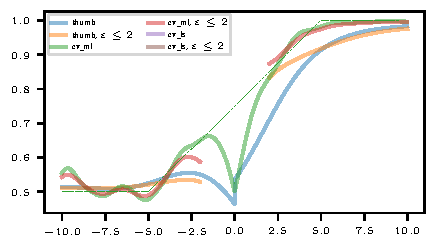
\includegraphics{plots/illustrative_examples/cond_prob_plot_bw_asym_butterfly}
        \caption{First dataset with asymmetric dependence.}
    \end{subfigure}
    \begin{subfigure}{.48\textwidth}
        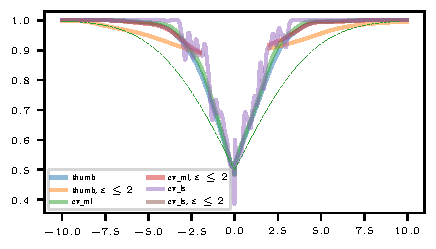
\includegraphics{plots/illustrative_examples/cond_prob_plot_bw_normal}
        \caption{Second dataset. }
    \end{subfigure}
    \caption{Resulting conditional trending plot for different bandwidth selection processes. Cross validation least squares takes a considerably larger computation time while yielding the results with best balance between smoothing and displaying local effects. The rule of thumb is the fastest method but tends to oversmooth. Cross validation least squares  }\label{fig:trending-cond-prob-bw}
\end{figure}


\subsection{Confidence intervals based on bootstrapping}\label{subsec:trending-bootstrap}

Confidence intervals can be issued to account for the estimation uncertainty of the measures above.
Bootstrapping confidence intervals are a nonparametric technique based on resampling~\parencite[for introductions see][]{Hesterberg2011,Bittmann2021}.
Whereas classical confidence intervals are computed from parametric assumptions on the underlying data, new samples are drawn with replacement from the dataset in bootstrapping.
The confidence interval is then computed based on the bootstrap samples.
We examine three methods for bootstrapping here: the intuitive percentile and the more sophisticated basic and \ac{bca} method.
In the \textit{percentile} approach, the confidence interval for level $\alpha$ is built directly from the bootstrap estimators' empirical distribution.
The \textit{basic} approach computes the confidence interval based on the non-bootstrapped estimate using the bootstrapped quantile deviations~\parencite{Davison1997}.
The \ac{bca} method modifies the quantiles of the empirical bootstrap distribution by a bias and an acceleration parameter~\parencite{Efron1987}.
Typically, the percentile approach needs larger datasets and provides an easy and fast estimate, while the \ac{bca} is computationally expensive but needs smaller datasets for reasonable confidence intervals.
The basic approach balances those two aims.
We compare the approaches in a small synthetic data study in the following with respect to their small-dataset behavior and their computation time.
We vary the number of available time steps $T$ to be a typical time-series value, such as 30 for daily data in a month, 52 for weekly data, 168, 365, 720, and 1024.
The considered datasets are again the ones outlined in Appendix~\ref{sec:app-trending-data-generation}, the first dataset with asymmetric dependence.
In the calculations, the \verb|scipy| package's implementation of bootstrap confidence intervals were used~\parencite{Virtanen2020}.
The prescribed confidence level is 90 \% and the number of bootstrap samples is $10,000$.
The share of confidence intervals covering the true values per method and $T$ are shown in Table~\ref{tab:trending_bootstrap}.
The true values of the accuracy are computed based on a dataset of size $10^9$, yielding 0.7501 and 0.7700 for the two datasets.
The computation times per method and dataset are shown in Figure~\ref{fig:trending_bootstrap_time}.
\todo[inline]{Add evaluation when computation is finished}

\begin{table}
    \centering
    \begin{subtable}{.48\textwidth}
        \begin{tabular}{llll}
\toprule
 & percentile & basic & bca \\
\midrule
30 & 0.84 (0.249) & 0.86 (0.250) & 0.91 (nan) \\
52 & 0.89 (0.194) & 0.89 (0.193) & 0.89 (0.198) \\
168 & 0.91 (0.109) & 0.90 (0.109) & 0.90 (0.110) \\
365 & 0.90 (0.074) & 0.90 (0.074) & 0.90 (0.074) \\
720 & 0.90 (0.053) & 0.90 (0.053) & 0.90 (0.053) \\
1024 & 0.90 (0.044) & 0.90 (0.044) & 0.89 (0.044) \\
\bottomrule
\end{tabular}

        \caption{First dataset}
    \end{subtable}\hspace{0.02\textwidth}
    \begin{subtable}{.48\textwidth}
        \begin{tabular}{llll}
\toprule
 & percentile & basic & BCa \\
\midrule
30 & 0.87 (0.243) & 0.88 (0.242) & 0.92 (0.249) \\
52 & 0.87 (0.188) & 0.89 (0.188) & 0.90 (0.192) \\
168 & 0.89 (0.106) & 0.90 (0.106) & 0.90 (0.107) \\
365 & 0.90 (0.072) & 0.90 (0.072) & 0.90 (0.072) \\
720 & 0.90 (0.052) & 0.90 (0.052) & 0.90 (0.052) \\
1024 & 0.89 (0.043) & 0.90 (0.043) & 0.90 (0.043) \\
\bottomrule
\end{tabular}

        \caption{Second dataset}
    \end{subtable}
    \caption{Proportion of bootstrapping confidence intervals covering the true value of trending ratio per method and sample size $T$. The average width of the confidence interval is listed in brackets.}
    \label{tab:trending_bootstrap}
\end{table}

\begin{table}
    \centering
    \begin{subfigure}{0.48\textwidth}
        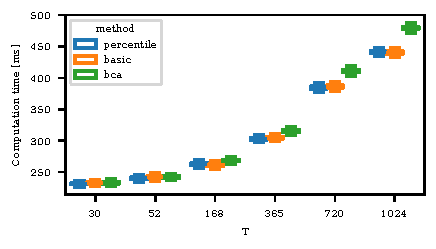
\includegraphics{plots/illustrative_examples/boxplot_comp_time_butterfly}
        \caption{First dataset}
    \end{subfigure}
    \begin{subfigure}{0.48\textwidth}
        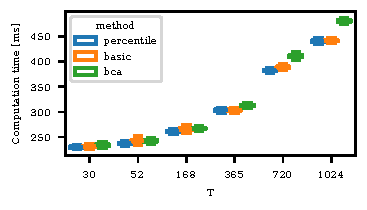
\includegraphics{plots/illustrative_examples/boxplot_comp_time_normal}
        \caption{Second dataset}
    \end{subfigure}
    \caption{Boxplot of the computation time of the different bootstrapping method and data set sizes $T$. The computation time refers to bootstrapping one confidence interval based upon $10,000$ values. Each boxplot reflects $10,000$ samples. The \ac{bca} method takes slighlty longer than the other two but the difference is neglectable.}
    \label{fig:trending_bootstrap_time}
\end{table}



In bootstrapping, the sample is assumed to be independent and identically distributed.
Thus, before applying bootstrapping methods, the strength of sequential dependence should be inspected, for example, by analyzing the autocorrelation and partial autocorrelation.
Bootstrapping focusing on time series data is covered in~\textcite{Hardle2003,Kreiss2012}, for example.